\documentclass{article}\usepackage[]{graphicx}\usepackage[]{xcolor}
% maxwidth is the original width if it is less than linewidth
% otherwise use linewidth (to make sure the graphics do not exceed the margin)
\makeatletter
\def\maxwidth{ %
  \ifdim\Gin@nat@width>\linewidth
    \linewidth
  \else
    \Gin@nat@width
  \fi
}
\makeatother

\definecolor{fgcolor}{rgb}{0.345, 0.345, 0.345}
\newcommand{\hlnum}[1]{\textcolor[rgb]{0.686,0.059,0.569}{#1}}%
\newcommand{\hlsng}[1]{\textcolor[rgb]{0.192,0.494,0.8}{#1}}%
\newcommand{\hlcom}[1]{\textcolor[rgb]{0.678,0.584,0.686}{\textit{#1}}}%
\newcommand{\hlopt}[1]{\textcolor[rgb]{0,0,0}{#1}}%
\newcommand{\hldef}[1]{\textcolor[rgb]{0.345,0.345,0.345}{#1}}%
\newcommand{\hlkwa}[1]{\textcolor[rgb]{0.161,0.373,0.58}{\textbf{#1}}}%
\newcommand{\hlkwb}[1]{\textcolor[rgb]{0.69,0.353,0.396}{#1}}%
\newcommand{\hlkwc}[1]{\textcolor[rgb]{0.333,0.667,0.333}{#1}}%
\newcommand{\hlkwd}[1]{\textcolor[rgb]{0.737,0.353,0.396}{\textbf{#1}}}%
\let\hlipl\hlkwb

\usepackage{framed}
\makeatletter
\newenvironment{kframe}{%
 \def\at@end@of@kframe{}%
 \ifinner\ifhmode%
  \def\at@end@of@kframe{\end{minipage}}%
  \begin{minipage}{\columnwidth}%
 \fi\fi%
 \def\FrameCommand##1{\hskip\@totalleftmargin \hskip-\fboxsep
 \colorbox{shadecolor}{##1}\hskip-\fboxsep
     % There is no \\@totalrightmargin, so:
     \hskip-\linewidth \hskip-\@totalleftmargin \hskip\columnwidth}%
 \MakeFramed {\advance\hsize-\width
   \@totalleftmargin\z@ \linewidth\hsize
   \@setminipage}}%
 {\par\unskip\endMakeFramed%
 \at@end@of@kframe}
\makeatother

\definecolor{shadecolor}{rgb}{.97, .97, .97}
\definecolor{messagecolor}{rgb}{0, 0, 0}
\definecolor{warningcolor}{rgb}{1, 0, 1}
\definecolor{errorcolor}{rgb}{1, 0, 0}
\newenvironment{knitrout}{}{} % an empty environment to be redefined in TeX

\usepackage{alltt}
\usepackage{amsmath} %This allows me to use the align functionality.
                     %If you find yourself trying to replicate
                     %something you found online, ensure you're
                     %loading the necessary packages!
\usepackage{amsfonts}%Math font
\usepackage{graphicx}%For including graphics
\usepackage{hyperref}%For Hyperlinks
\usepackage[shortlabels]{enumitem}% For enumerated lists with labels specified
                                  % We had to run tlmgr_install("enumitem") in R
\hypersetup{colorlinks = true,citecolor=black} %set citations to have black (not green) color
\usepackage{natbib}        %For the bibliography
\setlength{\bibsep}{0pt plus 0.3ex}
\bibliographystyle{apalike}%For the bibliography
\usepackage[margin=0.50in]{geometry}
\usepackage{float}
\usepackage{multicol}

%fix for figures
\usepackage{caption}
\newenvironment{Figure}
  {\par\medskip\noindent\minipage{\linewidth}}
  {\endminipage\par\medskip}
\IfFileExists{upquote.sty}{\usepackage{upquote}}{}
\begin{document}

\vspace{-1in}
\title{Lab 3 -- MATH 240 -- Computational Statistics}

\author{
  Sankalp Ojha \\
  Colgate University  \\
  Mathematics  \\
  {\tt sojha@colgate.edu}
}

\date{}

\maketitle

\begin{multicols}{2}
\begin{abstract}
Will fill out at the end of the lab once we are done with all the tasks.
\end{abstract}

\section{Introduction}
Through this lab, we will be exploring who contributed more to the song "Allentown". Was it The Front Bottoms or Manchester Orchestra? To answer the question at hand, we will analyze all the songs released, excluding all joint albums, live albums, and single releases contained in a full album or an Extended Play (EP), by both bands before Allentown. Through the analysis, we will aim to determine the style of each band which will allow us to compare Allentown's style with each band. The comparison will allow us to determine which band's style matches the most with Allentown, leading to the conclusion of which band contributed in a greater quantity.

\section{Methods}

\subsection{Making A batfile.txt}
To accomplish this lab, we will first need to create a \texttt{batfile.txt} file using the \texttt{R} package \texttt{stringr} \citep{stringr} which we can execute in the command line to produce a \texttt{.json} file. Using the \texttt{R} package \texttt{jsonlite} \citep{jsonlite} we will gather all relevant information needed, such as tempo in beats per minute, musical key or musical mode, to analyze the similarities between the each band's style and Allentown's style. 

To create the \texttt{batfile.txt} file, I downloaded all the given songs which were assorted by artist with a sub folder for each album. Each album folder contains all the songs in that given album. We retrieved the artist name, album name, and each track's name from the file path to create a file name for each song's \texttt{.json} file. Each song's file path and \texttt{.json} file name were pasted into an execuatble \texttt{batfile.txt} file which will be used to create the necessary \texttt{.json} file for each song.

\subsection{Gathering All Relevant Data}
Once we had all 181 \texttt{.json} files for each song, it was time to sift through all the data and gather all relevant information needed for our analysis. We also were provided with Essentia models which came in the form of a \texttt{.csv} file. The grand outcome of this portion of the lab is to sift through the data and create a new data frame with only the relevant information we will need for the final portion of the lab which will be to analyze the data. Cleaning up the data first requires combining similar variables into one average variable. For example, for the party measurement, we took an average of the \texttt{eff party} and \texttt{nn party} varibles to get a mean average party variable. We used this combining process for all the measurements we wanted to analyze at the end. The final step of compling all the relevant informantion was creating a new data frame which only cotained the necesary information such as artist, album, track, and all the new varibles we created.

\subsection{Merging The \texttt{.csv} Files}
The next portion of the lab involved merging our new data frame which we made with all the necessary information and a \texttt{.csv} file which contains information about the lyrics and personality types of the songs. We used the \texttt{R} function \texttt{merge()} to merge the \texttt{streaming music extractor} \texttt{.csv}, the new \texttt{.csv} we made, and the languge \texttt{.csv} file. The new merged dataframe will allow us to extract various pieces of information which we will be able to use for making graphs and plots for analyizng which band contributed more to the making of Allentown.

\section{Results}
In the appendix there are two violin plots which show a Relaxed V. Artist and timbreBright V. Artist plot. Relaxed and timbreBright are both varibles which measure different aspects on the songs. The merged \texttt{.csv} file will is our gateway to creating plots for the analysis portion of the lab.

\section{Discussion}
As can be seen in the Relaxed V. Artist plot, Manchester Orchestra is more leftward, whereas The Front Bottoms is more rightward. As can be seen in the timbreBright V. Artist plot, Manchester Orchestra is more in the center, whereas The Front Bottoms is more leftward. We will next need to analyze where Allentown falls on these graphs to make any predictions about which band contributed more.

%%%%%%%%%%%%%%%%%%%%%%%%%%%%%%%%%%%%%%%%%%%%%%%%%%%%%%%%%%%%%%%%%%%%%%%%%%%%%%%%
% Bibliography
%%%%%%%%%%%%%%%%%%%%%%%%%%%%%%%%%%%%%%%%%%%%%%%%%%%%%%%%%%%%%%%%%%%%%%%%%%%%%%%%
\vspace{2em}

\begin{tiny}
\bibliography{bib5}
\end{tiny}
\end{multicols}

%%%%%%%%%%%%%%%%%%%%%%%%%%%%%%%%%%%%%%%%%%%%%%%%%%%%%%%%%%%%%%%%%%%%%%%%%%%%%%%%
% Appendix
%%%%%%%%%%%%%%%%%%%%%%%%%%%%%%%%%%%%%%%%%%%%%%%%%%%%%%%%%%%%%%%%%%%%%%%%%%%%%%%%
\newpage
\onecolumn
\section{Appendix}

\begin{figure}[H]
\begin{center}
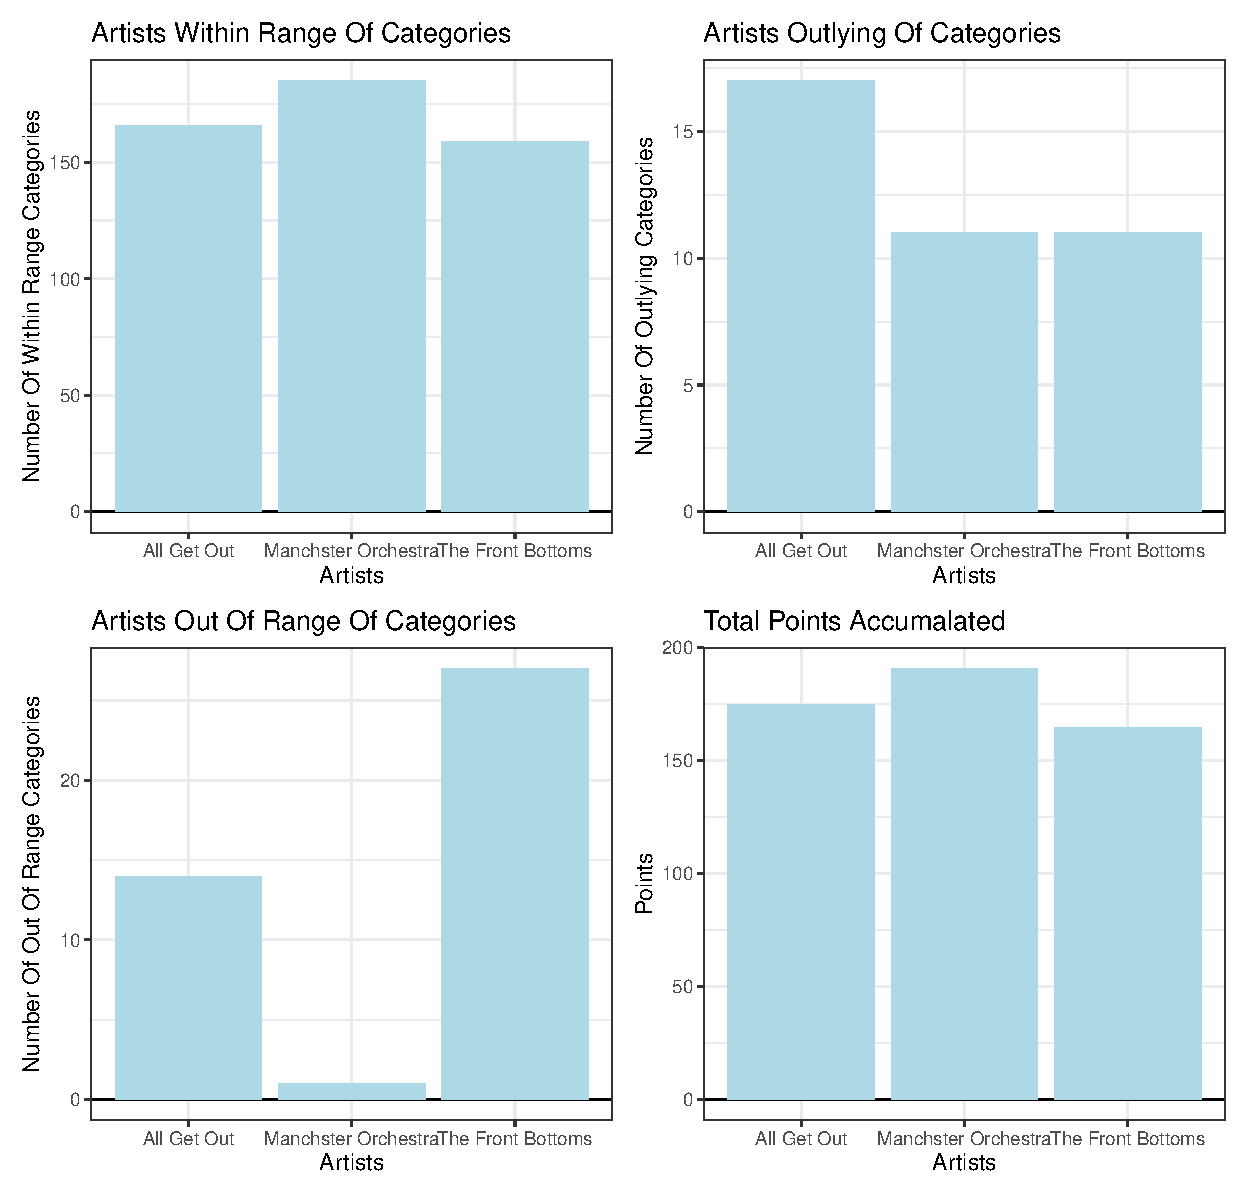
\includegraphics[scale=0.75]{Rplot.pdf}
\caption{Relaxed V. Artist}
\label{plot5}
\end{center}
\end{figure}

\begin{table}[ht]
\centering
\begin{tabular}{rlrrrr}
  \hline
 & artists & count.in.range & count.outlying & count.out.range & points \\ 
  \hline
1 & All Get Out & 166.00 & 17.00 & 14.00 & 174.50 \\ 
  2 & Manchster Orchestra & 185.00 & 11.00 & 1.00 & 190.50 \\ 
  3 & The Front Bottoms & 159.00 & 11.00 & 27.00 & 164.50 \\ 
   \hline
\end{tabular}
\end{table}

\end{document}
